In this section we will present what it means for a \verb|par| site to be
worthwhile. We do this by measuring the \emph{health} of each \verb|par| site.

The runtime system provides us with a variety of statistics about threads and
the \verb|par|s that sparked them. However, our current approach focuses on
reduction count as a guide to determine which \verb-par- sites are beneficial
to the program.  The reasoning is simple; our motivation for parallelism is to
do more work at once while ensuring that each bit of work done by a thread
makes up for the cost of creating and managing that thread, so measuring the
amount of work undertaken by each thread is the most direct measure of this
desirable property.

\begin{figure}
  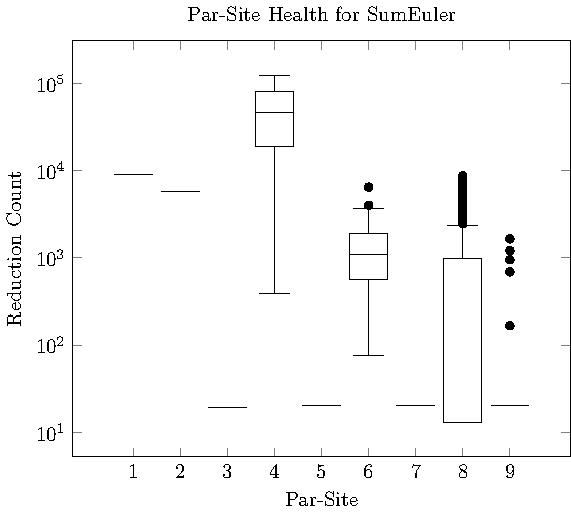
\includegraphics[width=\linewidth]{Informed/Figures/threadhealth.pdf}
\caption{Statistics on the number of reductions carried out by the threads a
\texttt{par} site sparks off}
\label{fig:sumHist}
\end{figure}

Because we record how productive each thread in a program is and we keep track
of which \verb-par- site created each thread, we can easily visualise how
useful each \verb-par- site is. Figure \ref{fig:sumHist} gives an overview of
the health of each \verb-par- site for the \verb|SumEuler| benchmark. The plot
shows us the statistics for this data with the median (line), inter-quartile
range (IQR, box), and $\pm1.5 * $IQR (whiskers).  Statistical outliers are
shown as independent points. The \verb-par-sites that only show a line as their
plot either have only one child thread (the case for \verb-par--site 1) or have
little variance in the distribution of reduction counts.

Even by just plotting this information we gain a much better understanding of
\verb|SumEuler|'s parallel behaviour. Much like using Threadscope
\citep{Jones2009Tuning}, having this information helps the programmer (and the
compiler in our case) make better decisions about where to look for performance
improvements. In the case of the profile shown in Figure \ref{fig:sumHist} we
can clearly see that some \verb|par| sites do not spark hard-working threads.

Additionally, we can see that the variance between the productivity of the
threads sparked by a \verb|par| site can be quite high (\verb|par| site \#4
sparks some threads that perform hundreds of reductions and some that
perform hundreds of thousands of reductions).

We define a \verb|par|'s \textbf{health} as the \emph{mean} of the reduction
counts for \emph{all} the threads sparked off by the \verb|par| site in
question. This simple view provides a rough estimate of how worthwhile a
\verb|par| site is overall while requiring very little computation on its own.
Another important aspect of this measure is that \verb|par| site health is more
of a \emph{relative} measure than an absolute measure. Trying to define what is
healthy or not healthy for all programs is difficult. Instead we aim to rank a
\verb|par|'s health as compared to the other \verb|par|'s in a program.

For the \verb|SumEuler| program's \verb|par| sites as shown in Figure
\ref{fig:sumHist}, this means that \verb|par| site numbers 3, 5, 7, 8, and 9
are less healthy than site numbers 1, 2, 4, and 6.
